\chapter{p3 = 24 (3 graphs)}
\newpage\begin{figure}
  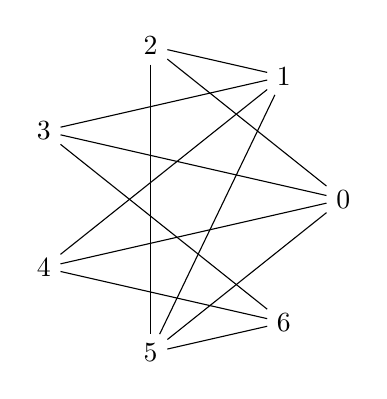
\begin{tikzpicture}
      \draw
        (0.0:2) node (0){0}
        (51.429:2) node (1){1}
        (102.857:2) node (2){2}
        (154.286:2) node (3){3}
        (205.714:2) node (4){4}
        (257.143:2) node (5){5}
        (308.571:2) node (6){6};
      \begin{scope}[-]
        \draw (0) to (2);
        \draw (0) to (3);
        \draw (0) to (4);
        \draw (0) to (5);
        \draw (1) to (2);
        \draw (1) to (3);
        \draw (1) to (4);
        \draw (1) to (5);
        \draw (2) to (5);
        \draw (3) to (6);
        \draw (4) to (6);
        \draw (5) to (6);
      \end{scope}
    \end{tikzpicture}
\end{figure}
\begin{itemize}
\item signature: 011110111100010001011
\item g: Graph with 7 nodes and 12 edges
\item order: 7
\item size: 12
\item max degree: 4
\item degrees: 3,3,3,3,4,4,4
\item is tree: 0
\item is bipartite: 0
\item has bridge: 0
\item is chordal: 0
\item is complete: 0
\item min cycle basis weight: 22
\item min cycle basis size: 6
\item diameter: 2
\item radius: 2
\item is eulerian: 0
\item is planar: 0
\item number of faces: 7
\item is regular: 0
\item p3: 24
\item p4: None
\item property hash: 5ad017f1c54925e4cf97d5f930fbf12473f7320d8daecdb278dddccc9da3b13c
\end{itemize}
\newpage
\begin{figure}
  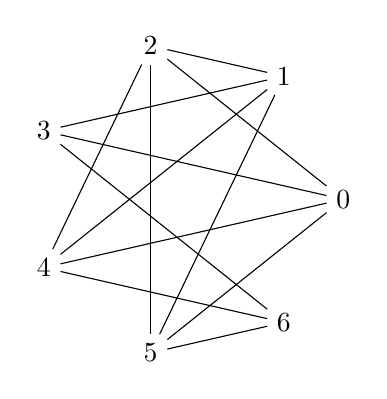
\begin{tikzpicture}
      \draw
        (0.0:2) node (0){0}
        (51.429:2) node (1){1}
        (102.857:2) node (2){2}
        (154.286:2) node (3){3}
        (205.714:2) node (4){4}
        (257.143:2) node (5){5}
        (308.571:2) node (6){6};
      \begin{scope}[-]
        \draw (0) to (2);
        \draw (0) to (3);
        \draw (0) to (4);
        \draw (0) to (5);
        \draw (1) to (2);
        \draw (1) to (3);
        \draw (1) to (4);
        \draw (1) to (5);
        \draw (2) to (4);
        \draw (2) to (5);
        \draw (3) to (6);
        \draw (4) to (6);
        \draw (5) to (6);
      \end{scope}
    \end{tikzpicture}
\end{figure}
\begin{itemize}
\item signature: 011110111100110001011
\item g: Graph with 7 nodes and 13 edges
\item order: 7
\item size: 13
\item max degree: 4
\item degrees: 3,3,4,4,4,4,4
\item is tree: 0
\item is bipartite: 0
\item has bridge: 0
\item is chordal: 0
\item is complete: 0
\item min cycle basis weight: 24
\item min cycle basis size: 7
\item diameter: 2
\item radius: 2
\item is eulerian: 0
\item is planar: 0
\item number of faces: 8
\item is regular: 0
\item p3: 24
\item p4: None
\item property hash: 37b3a21dbd8c42d86abd8753c3b375b36e368a8af314819bf7a10a46bc0931cf
\end{itemize}
\newpage
\begin{figure}
  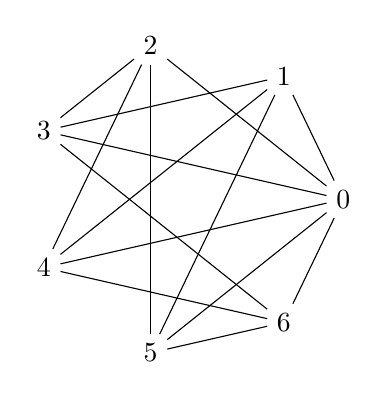
\begin{tikzpicture}
      \draw
        (0.0:2) node (0){0}
        (51.429:2) node (1){1}
        (102.857:2) node (2){2}
        (154.286:2) node (3){3}
        (205.714:2) node (4){4}
        (257.143:2) node (5){5}
        (308.571:2) node (6){6};
      \begin{scope}[-]
        \draw (0) to (1);
        \draw (0) to (2);
        \draw (0) to (3);
        \draw (0) to (4);
        \draw (0) to (5);
        \draw (0) to (6);
        \draw (1) to (3);
        \draw (1) to (4);
        \draw (1) to (5);
        \draw (2) to (3);
        \draw (2) to (4);
        \draw (2) to (5);
        \draw (3) to (6);
        \draw (4) to (6);
        \draw (5) to (6);
      \end{scope}
    \end{tikzpicture}
\end{figure}
\begin{itemize}
\item signature: 111111011101110001011
\item g: Graph with 7 nodes and 15 edges
\item order: 7
\item size: 15
\item max degree: 6
\item degrees: 4,4,4,4,4,4,6
\item is tree: 0
\item is bipartite: 0
\item has bridge: 0
\item is chordal: 0
\item is complete: 0
\item min cycle basis weight: 27
\item min cycle basis size: 9
\item diameter: 2
\item radius: 1
\item is eulerian: 1
\item is planar: 0
\item number of faces: 10
\item is regular: 0
\item p3: 24
\item p4: None
\item property hash: 7b409fcaf92e6e06efc2dce59d8f76ea639eb290391050d423f11c505213fe3e
\end{itemize}
\newpage
